% Left frame
%%%%%%%%%%%%%%%%%%%%
\begin{figure}
	\hfill
	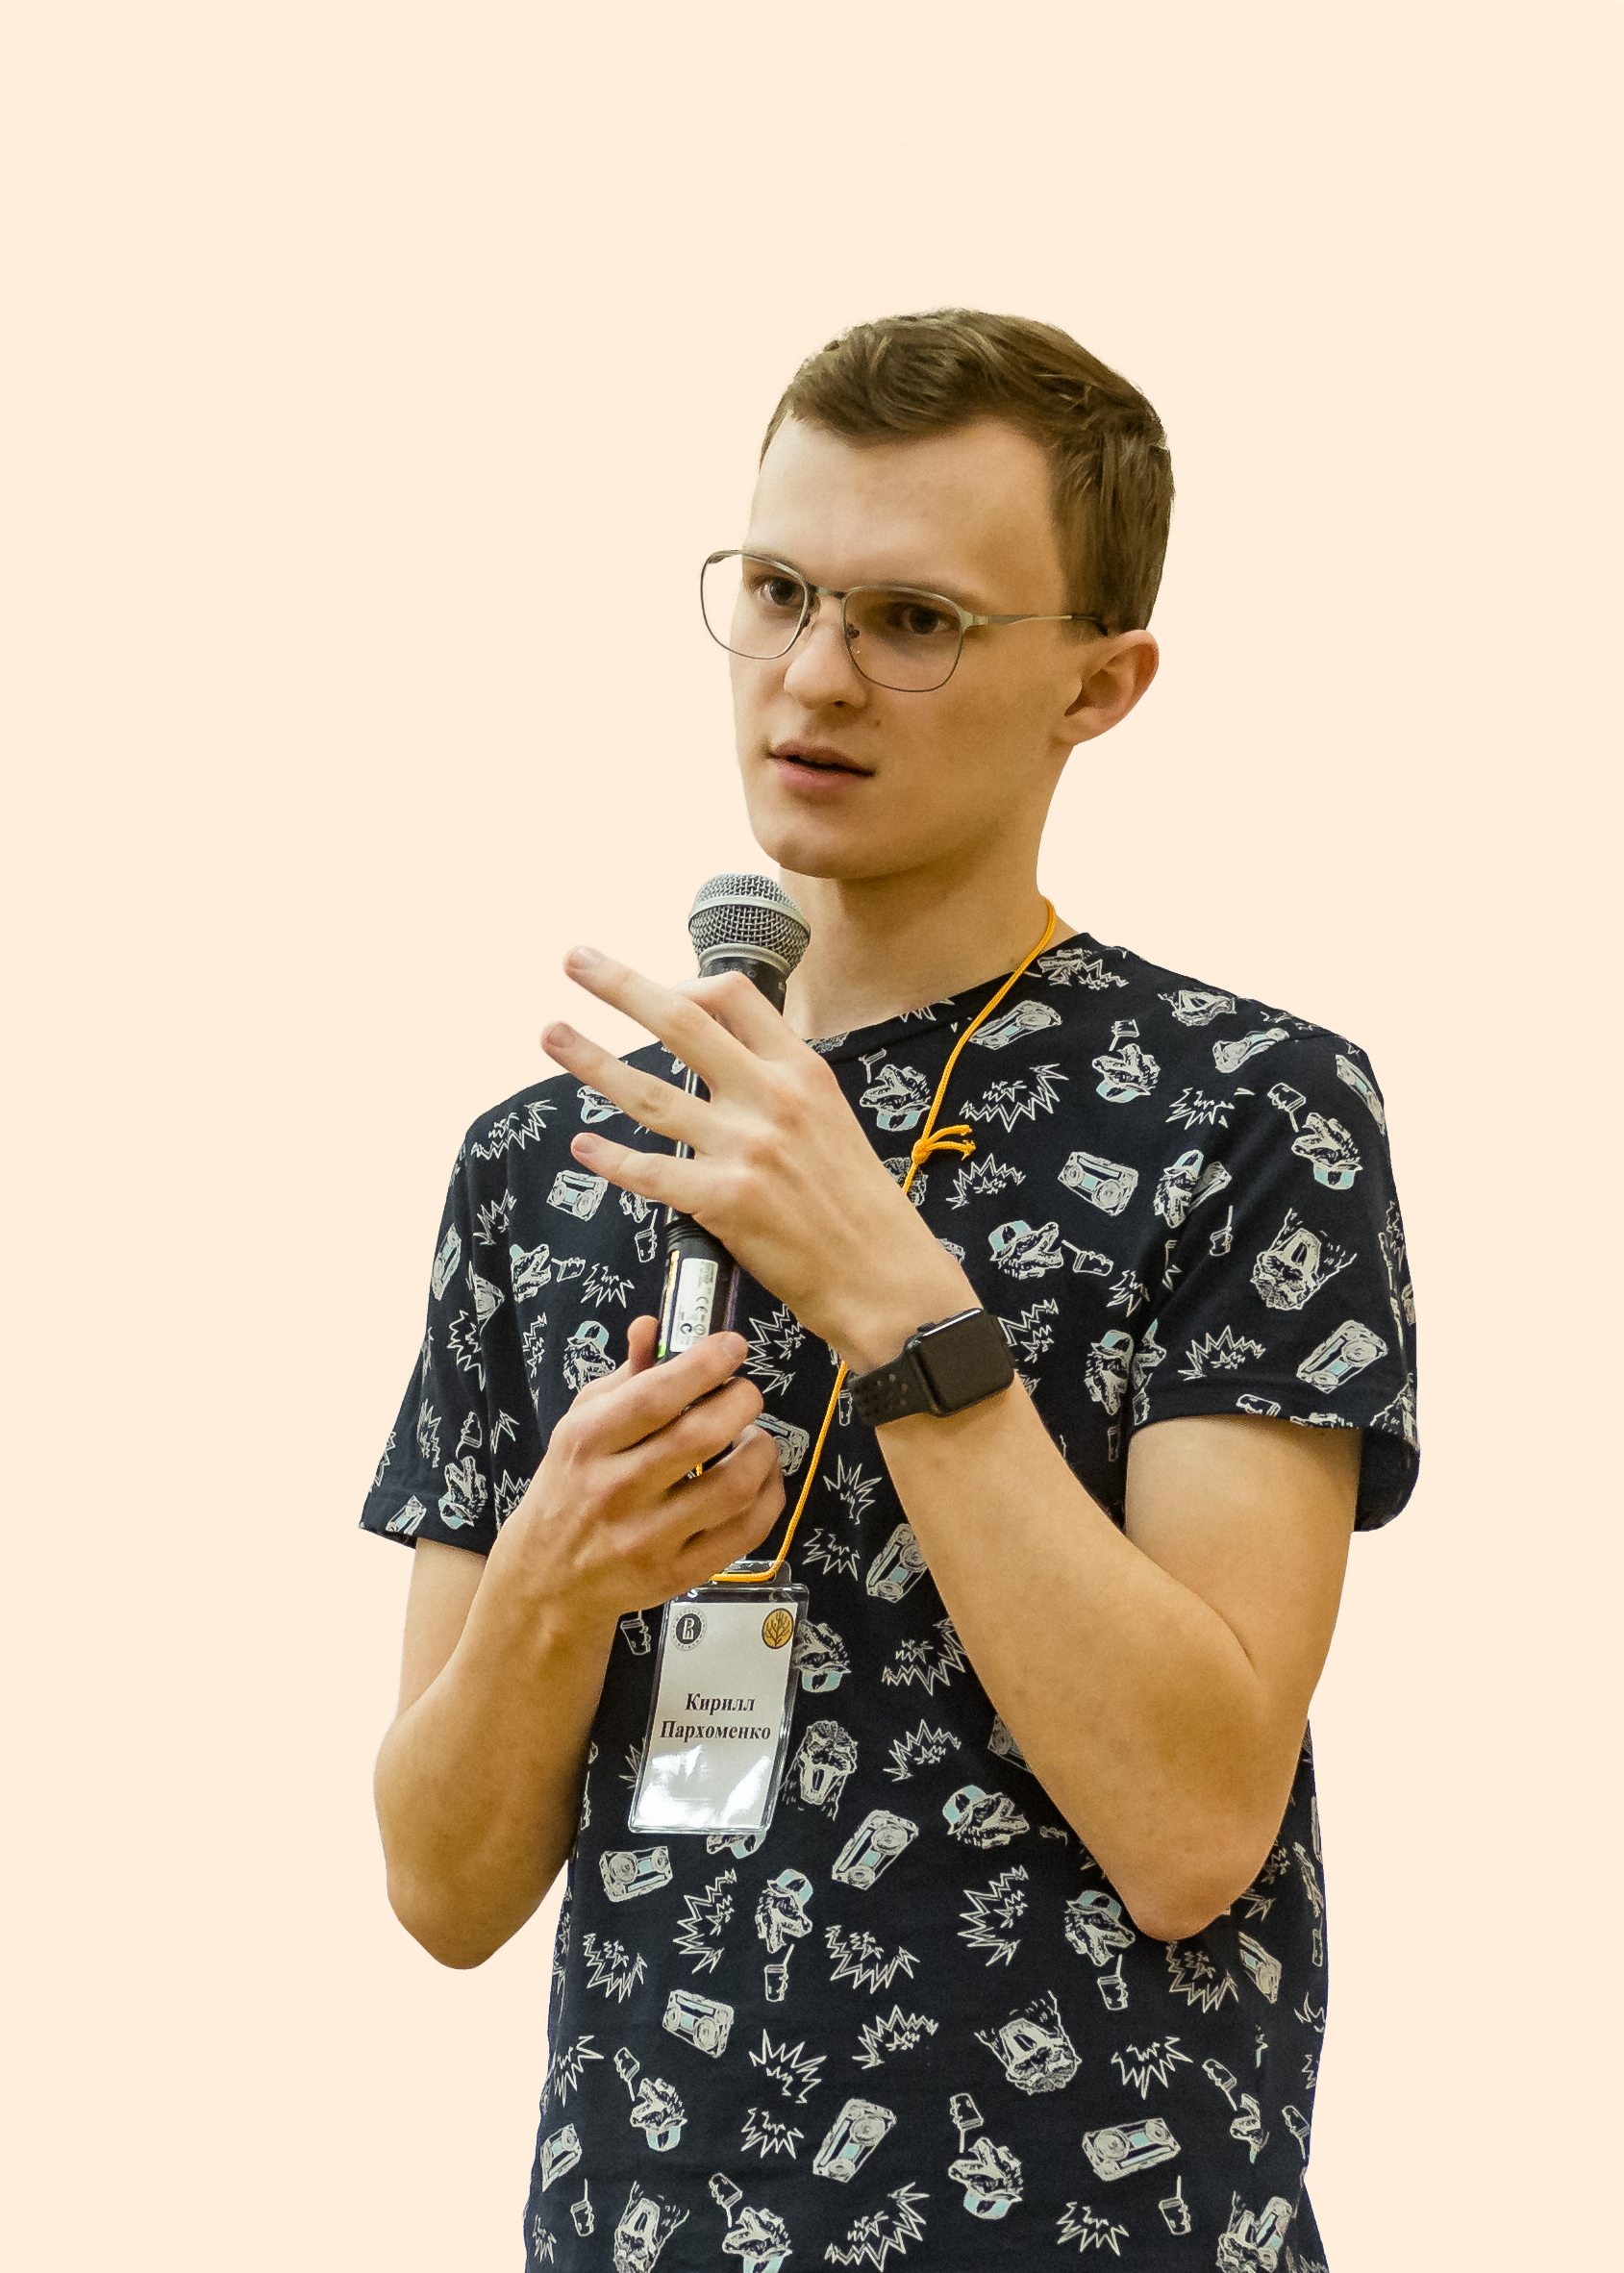
\includegraphics[width=1.0\columnwidth]{photo}
	\vspace{-7cm}
\end{figure}

\begin{flushright}\small
	
\end{flushright}\normalsize
\framebreak



% Right frame
%%%%%%%%%%%%%%%%%%%%
\Huge\bfseries\ {{\color{Cyan} Kirill} {\color{Black} Parhomenko}} \\
\NegativeSmallSep

\normalsize\bfseries Java Developer, bachelor \\
\small {\normalfont 23 y.o. Orenburg, Russia}

\normalsize\normalfont
\SmallSep


% Contacts
\begin{multicols}{2}
	\begin{compactitem}[\color{Cyan}$\circ$]
		\item\small \url{https://t.me/kirill_nk};
		\item\small \href{mailto:kirill.parhomenko@gmail.com}{kirill.parhomenko@gmail.com}.
		\item\small \url{https://github.com/sigseg5};
	\end{compactitem}
\end{multicols}

\SmallSep



% About me
I have been interested in information technology for most of my life, my main interests are programming, privacy and confidentiality tools and Computer Science.

\Sep



% Skills
\CVSection{Skills}

\CVItem{Languages I speak}
\begin{multicols}{3}
	\begin{compactitem}[\color{Cyan}$\circ$]
		\item Russian, native;
		\item English, B1.
	\end{compactitem}
\end{multicols}

\SmallSep

\CVItem{Programming and other Languages}
\begin{multicols}{3}
	\begin{compactitem}[\color{Cyan}$\circ$]
		\item Java Core;
		\item Kotlin Core;
		\item Base SQL;
		\item Python;
		\item bash;
		\item Swift;
		\item SASS;
		\item PUG;
		\item HTML5/CSS3;
		\item JS;
		\item \LaTeX.
		\item \ldots
	\end{compactitem}
\end{multicols}

\SmallSep

\CVItem{Technologies}
\begin{multicols}{3}
	\begin{compactitem}[\color{Cyan}$\circ$]
		\item Open Source \heart\
		\item Git;
		\item Docker;
		\item DigitalOcean;
		\item Parallel Computing;
		\item Basic ML;
		\item IntelliJ based IDEs;
		\item Figma, Sketch;
		\item Affinity Photo.
		\item \ldots
	\end{compactitem}
\end{multicols}

\Sep



% Experience
\CVSection{Experience}

\CVItem{November 2020 - present} \\
at \textit{Freelance}
as \textit{Junior Java Developer}
\SmallSep

In October, I finished some courses and move to Java Backend development, where I do some simple web projects.
\SmallSep

\texttt{Java Core / Java 8 / Docker}
\SmallSep

\CVItem{February 2019 - May 2019} \\
at \textit{Freelance}
as \textit{Swift Developer}
\SmallSep

After taking courses on "iOS and Swift development" in end of 2018, I started working at small projects for iOS.
\SmallSep

\texttt{Swift / Realm database / UIKit}
\SmallSep

\CVItem{February 2018 - February 2019} \\
at \textit{CreaWave}
as \textit{Middle Frontend Developer;}
\SmallSep

After some courses and practice I get Middle Frontend Developer role in this company, I moved to modern PUG, SCSS and React development.
\SmallSep

\texttt{PUG / SCSS / JavaScript / NodeJS / React / BEM }
\SmallSep

\CVItem{December 2017} \\
at \textit{CreaWave}
as \textit{Junior Frontend Developer}
\SmallSep

In December, I get a first job as Frontend Developer, where I do semantic and cross-browser web development with modern HTML5,  CSS3 and JavaScript principles.
\SmallSep

\texttt{HTML5 / CSS3 / JS}

\clearpage
\framebreak
\framebreak



% Education
\CVSection{Education}
\CVItem{2016 - 2020} \\
at \textit {Orenburg State University}

\SmallSep

Faculty of Mathematics and Information Technology, specialty computer science and computer engineering,  bachelor's honours degree, grade point average 4.95. I actively participated in the social life of the university, attending olympiads, hackathons, and conferences.

\SmallSep

\CVItem{2014 - 2016} \\
at \textit {Orenburg, Lyceum № 3, Physics and Mathematics class;}
\SmallSep

Since ninth grade, I've been getting a math education. In addition, I actively studied Computer Science.

\SmallSep

\CVItem{2005 - 2014} \\
at \textit {Orenburg, Lyceum № 3.}

\Sep



% Courses
\CVSection{Courses}
\begin{multicols}{2}
	\begin{compactitem}[\color{Cyan}$\circ$]
		\item\footnotesize Professional HTML, CSS, level 1 \\
		by \footnotesize{HTML Academy;}
		
		\item\footnotesize Professional HTML, CSS, level 2 \\
		by \footnotesize{HTML Academy;}
		
		\item\footnotesize Introduction to Linux \\
		by \footnotesize{Stepik.org, Bioinformatics Institute}
		
		\item\footnotesize Git basics \\
		by \footnotesize{Stepik.org, Mark Zaslavskiy;}
		\vfill\columnbreak
		
		\item\footnotesize Programming in Python \\
		by \footnotesize{Stepik.org, Bioinformatics Institute;}
		
		\item\footnotesize Developing Android applications on Kotlin \\
		by \footnotesize{Stepik.org;}
		
		\item\footnotesize Introduction to the Kotlin JVM \\
		by \footnotesize{Stepik.org.}
		
		\item \ldots
		
	\end{compactitem}
\end{multicols}

\Sep



% Hackathons
\CVSection{Hackathons}

\CVItem{BreakPoint Hackathon} \\
by \textit{BreakPoint, Ufa}
on \textit{March 23 2019}
\SmallSep

\footnotesize My first hackathon experience was Breakpoint, a 36-hour Russian hackathon.

\footnotesize Our team took 2nd place. We developed a chat-bot for solving user support tasks using neural networks for Directum company;
\SmallSep

\texttt{Python / Django / Machine Learning / Sketch}

\SmallSep

\CVItem{Hack.Moscow v3.0} \\
by \textit{Russian Hackers, Russia}
on \textit{25-27 October 2019}
\SmallSep

This was my first international hackathon, lasting 36 hours.

Our team decided to take Data Visualization track by Transparency International. We came up with an idea that helps citizens to know their officials in form of a game, that we called Chinder. 
We could not quite present a polished product, but we had a lot of fun and gained a lot of experience;

\texttt{Java / Android Studio / Figma}

\SmallSep

\CVItem{Case-championship McKinsey Business Diving 2020} \\
by \textit{McKinsey, Online}
on \textit{March 1-10 2020}
\SmallSep

My first case-championship experience.

Our team chose the theme "Strategy for the Development of Moscow Transport. We conducted a systematic analysis and hypothesized directions for infrastructure development;

\SmallSep

%\clearpage
%\framebreak
%\framebreak


\CVItem{Junction Hackathon} \\
by \textit{Major League Hacking, Online}
on \textit{November 6-8 2020}
\SmallSep

At the international Junction hackathon, our team solved the "Where to eat with my hacker team optimizer" challenge from Aito.ai. We didn't make much progress, but it was an amazing experience.

\texttt{aito.ai / Python / Kotlin / MathCad}

\SmallSep

\Sep
